\documentclass[
  % all of the below options are optional and can be left out
  % course name (default: 2IL50 Data Structures)
  course = {{DS12E Clustering Algorithms}},
  % quartile (default: 3)
  quartile = {{2}},
  % assignment number/name (default: 1)
  assignment = 2,
  % student name (default: Some One)
  name = {{Michael Darmanis ; Vasilios Venieris}},
  % student number, NOT S-number (default: 0123456)
  studentnumber = {{7115152200004 ; 7115152200017}},
  % student email (default: s.one@student.tue.nl)
  email = {{mdarm@di.uoa.gr ; vvenieris@di.uoa.gr}},
  % first exercise number (default: 1)
  firstexercise = 1
]{aga-homework}

\begin{document}

\section{Introduction}

The main goal of this report\footnote{as stated at \url{https://www.kaggle.com/rohan0301/unsupervised-learning-on-country-data}} is to provide recommendations to the CEO of HELP International on how to allocate the organisation's resources in a strategic and effective manner, based on the identification of countries in need of development aid. This will be achieved through the implementation of a clustering analysis on a country data set using \matlab. The analysis will consist of several stages, including the exploration of the data's characteristics and patterns, the selection and transformation of relevant features, the selection of appropriate clustering algorithms, the execution of these algorithms, and the characterization of the resulting clusters.

The initial stage of the analysis involves the examination of the individual features of the data, including their data type and range of values, as well as the distribution of these values. The relationships between different features will also be considered. Following this, relevant features will be selected and transformed in order to make their values comparable. Based on the characteristics of the data and the desired properties of the clusters, the appropriate clustering algorithms will then be chosen. These algorithms will then be executed with different parameter-values in order to identify persistent clusters. Finally, the clusters will be characterised based on the values of the features within each cluster.

\section{``Feeling the data''}\label{sec:feel}

In this part of the analysis, characteristics of each individual feature in the dataset were examined in order to gain a better understanding of its nature. This involved determining the data type and range of values for each feature, as well as generating histograms to visualize the distribution of values. The mean and standard deviation were also calculated for each feature.

\begin{verbatim}
Feature       Type      Range                          Mean        Std Dev    
-----------   --------  -----------------------------  ----------- -----------
 child_mort   float     [      2.6000,     208.0000]      38.2701      40.3289
 exports      float     [      0.1090,     200.0000]      41.1090      27.4120
 health       float     [      1.8100,      17.9000]       6.8157       2.7468
 imports      float     [      0.0659,     174.0000]      46.8902      24.2096
 income       float     [    609.0000,  125000.0000]   17144.6886   19278.0677
 inflation    float     [     -4.2100,     104.0000]       7.7818      10.5707
 life_expec   float     [     32.1000,      82.8000]      70.5557       8.8932
 total_fer    float     [      1.1500,       7.4900]       2.9480       1.5138
 gdpp         float     [    231.0000,  105000.0000]   12964.1557   18328.7048
\end{verbatim}

The linear dependence between each feature and all the others was calculated using the Pearson correlation coefficient in order to gain insight into the relationships between different features in the data set. Additionally, standard score normalization and min-max feature scaling normalization were performed. The linear dependence between the transformed features were calculated in each case.
        
\begin{figure}[htbp]

\centering
\begin{subfigure}{0.4\textwidth}
    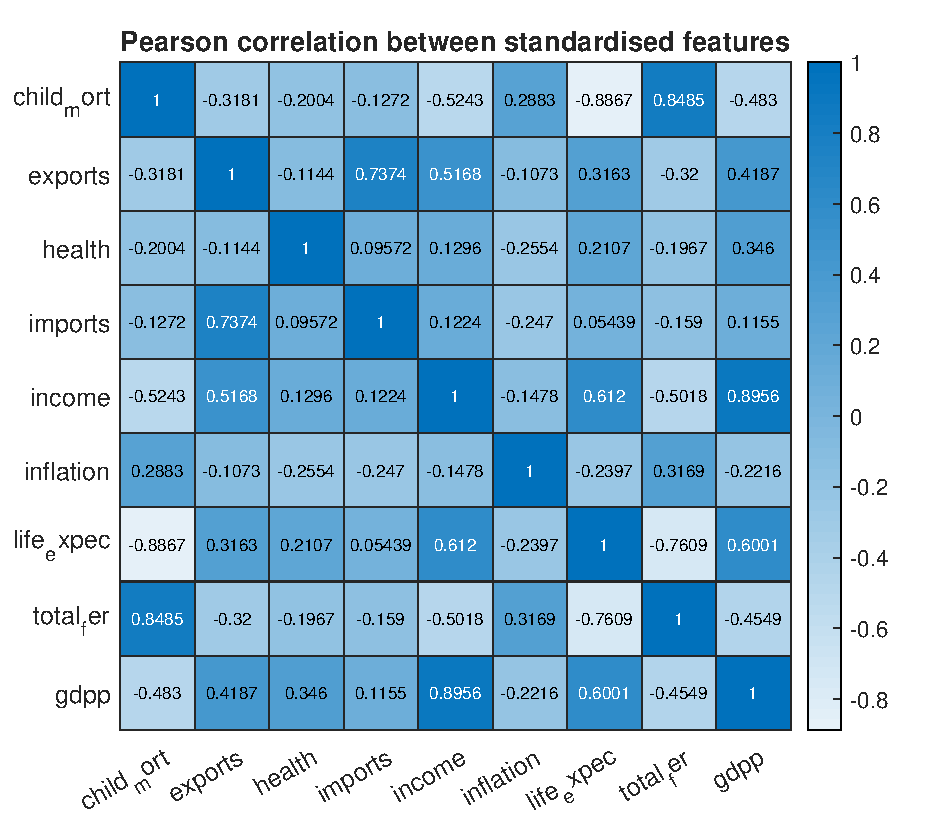
\includegraphics[width=\textwidth]{corr2}
    \caption{Standardised features.}
    \label{fig:first}
\end{subfigure}
\hfill
\begin{subfigure}{0.4\textwidth}
    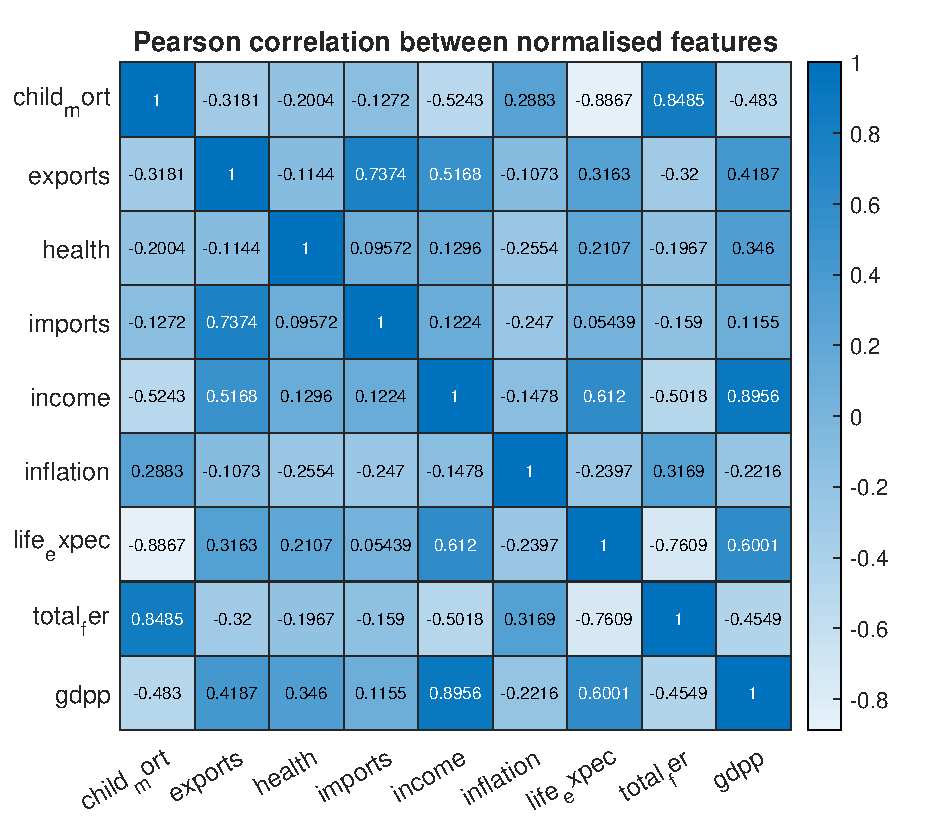
\includegraphics[width=\textwidth]{corr3}
    \caption{Min-max normalised features.}
    \label{fig:second}
\end{subfigure}
\hfill
\begin{subfigure}{0.4\textwidth}
    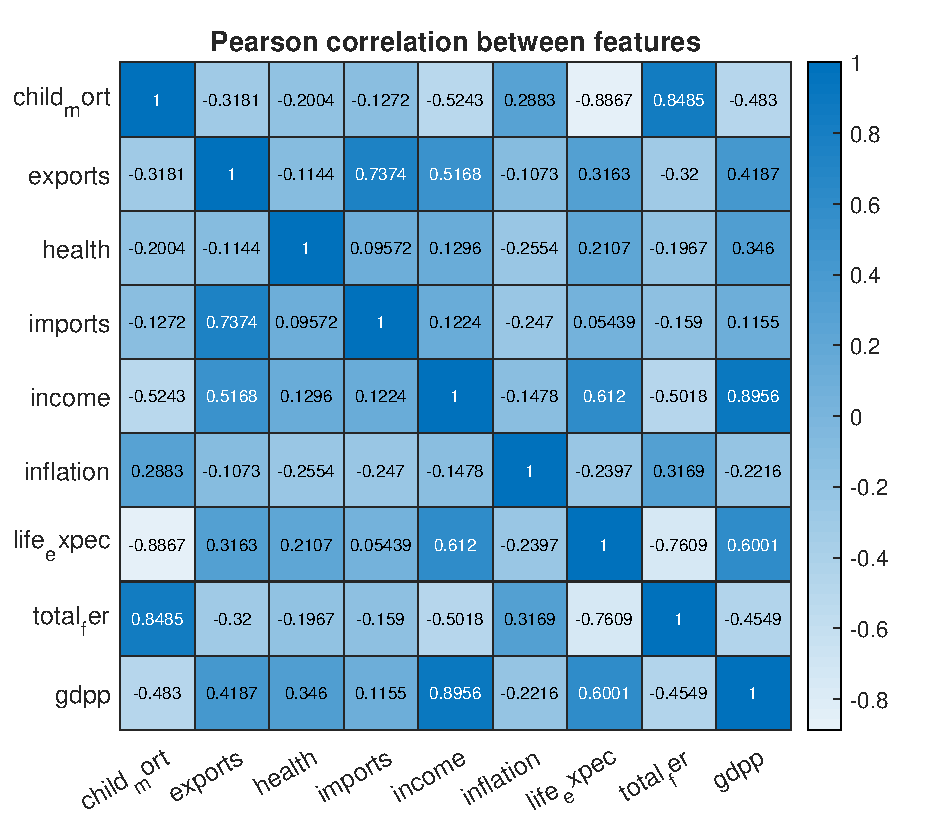
\includegraphics[width=\textwidth]{corr1}
    \caption{Raw features.}
    \label{fig:third}
\end{subfigure}
        
\caption{Correlation matrices between features.}
\label{fig:figures}

\end{figure}

It is evident in Figure~\ref{fig:figures} that linear relationships between features are not affected by the transformations. Pearson's correlation measures the linear component of association so it comes to no surprise that linear transformations of data (like mim-max normalisation and standardisation) did not affect the correlations between the features.

In Figure~\ref{fig:hist} it can readily be observed that the feature \texttt{life\textunderscore expec} exhibits a negative skew in its distribution, while the \texttt{health} exhibits a normal distribution. On the other hand, all other measured quantities show a positive skew in their distributions. It should be noted that the distribution of the categorical feature ``country'', which consists solely of text data and exhibits the same number of unique values as the total length of the data set, was not analysed since it makes little sense to do so.

\begin{figure}[htbp]
	\centering
	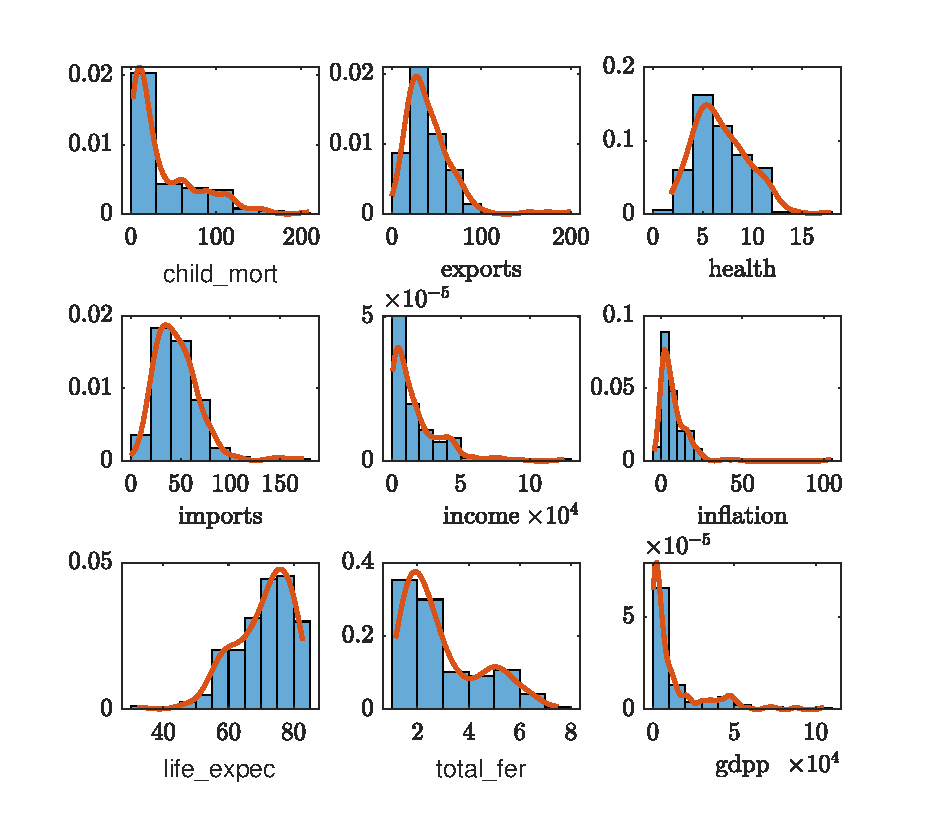
\includegraphics[scale=0.8]{histogram}
	\caption{Histograms and distributions of features}
	\label{fig:hist}
\end{figure}

The analysis of the dataset also reveals several relationships between features. The relationship between child mortality and economic conditions is of particular significance, as the data indicates that child mortality tends to increase as income, gross domestic product (GDP), and exports decrease. Inflation also appears to have a negative impact on child mortality. This suggests that economic factors, such as income and GDP, may be influential in determining child mortality rates. The relationship between exports and other economic indicators is also noteworthy, as an increase in exports tends to lead to an increase in GDP, income, and imports, implying that exports may be a key contributor to economic growth.

In addition, the data suggests that spending on health has a positive effect on life expectancy and a negative effect on child mortality. Higher levels of income and GDP are correlated with higher life expectancy and lower child mortality, indicating a possible relationship between these factors and spending on health. Furthermore, high levels of inflation appear to be detrimental to economic conditions, as they have a negative effect on various economic indicators, including income, GDP, and total fertility rate. Finally, the data suggests that higher life expectancy is correlated with lower total fertility rates, a relationship that may be influenced by factors such as GDP and spending on health.

\section{Feature selection/transformation}\label{sec:feature}

Based on the aformentioned data relationships, it is clear that some features are closely related to specific categories, namely: health, trade, and finance. Therefore, features will be grouped up into these categories and then normalised using a min-max scheme. The three categories of features in the dataset are: health (child mortality, health, life expectancy, total fertility rate), trade (imports, exports), and finance (income, inflation, GDP).

By combining multiple features into fewer ones facilitates the comprehension of relationships between different features and provides a more intuitive understanding of the data. It also captures broader or more general relationships in the data, and it may be possible to improve the generalisability of the clustering results to new, unseen data.

Additionally, by creating new features that capture more relevant or subtle relationships in the data, it may be possible to improve the performance of the clustering algorithm itself.

\section{Selection and execution of the clustering algorithms}\label{sec:execute_clusters}

After normalising and combining \& renormalising the data, the k-means clustering algorithm was used for performing the clustering analysis in order to effectively group countries in terms of their needs. The k-means algorithm is a popular choice for clustering due to its simplicity and efficiency, making it well-suited for large datasets (not that ours is, at this point anyway). Additionally, the algorithm produces clear and distinct clusters, which can be beneficial when attempting to partition the countries into groups. Overall, the use of k-means clustering in this context can provide valuable insights and aid in the strategic allocation of resources.

Determining the appropriate number of initial clusters in a k-means clustering operation can be achieved through the use of various measures such as the ``elbow method'' or the variance-ratio criterion\cite{calinski}. The ``elbow method'' for approximating the correct value of k is to run the algorithm for increasing values of k, until there is a minimal decrease in the chosen measure of cluster cohesion (the cost function in our case) between two values\cite{leskovec2020mining}. Alternative measures such as the Bayesian Information Criterion and Gap statistics are also suggested as preferable options\cite{schubert}. It is important to note that the ``elbow method'', which involves identifying a point of inflection in a plot of the measure of cluster cohesion versus k, has been criticized in the literature \parencites{milligan}{ketchen} and should, generally speaking, be avoided.

\begin{figure}[htbp!]
\centering
\begin{subfigure}{0.45\textwidth}
    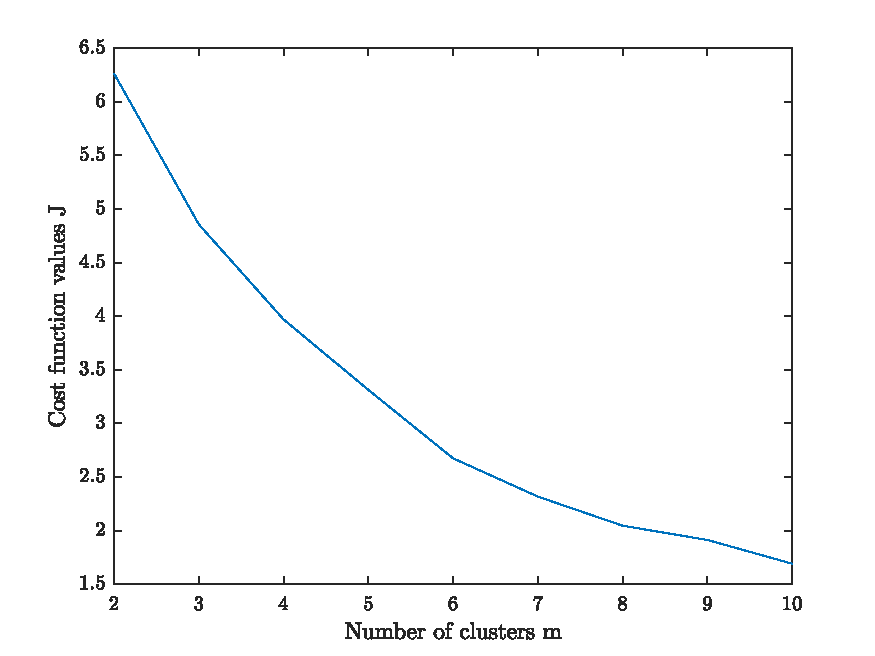
\includegraphics[width=\textwidth]{elbow}
    \caption{``Elbow'' method.}
    \label{fig:elbow}
\end{subfigure}
\hfill
\begin{subfigure}{0.45\textwidth}
    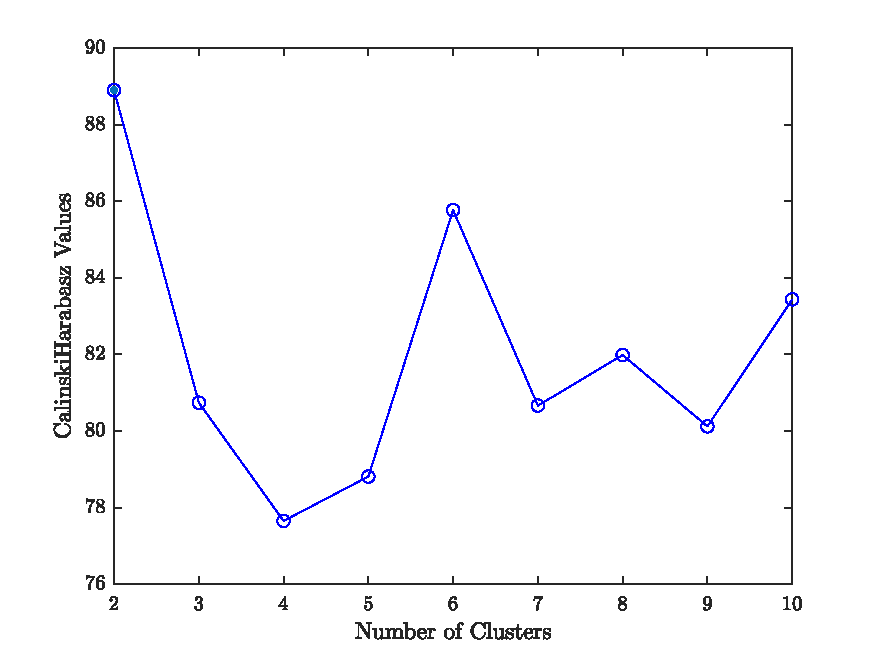
\includegraphics[width=\textwidth]{eval}
    \caption{Variance-ratio criterion.}
    \label{fig:eval}
\end{subfigure}
        
\caption{Picking the right number of initial clusters k.}
\label{fig:k-init}
\end{figure}

Both the ``elbow method'' (see Figure~\ref{fig:elbow}) and the variance-ratio criterion (see Figure~\ref{fig:eval}) agreed that the hidden structure underlying the data was expressed in three clusters. The the k-means algorithm was initialised using three clusters.

In order to pick initial points that have a good chance of being in different clusters, k-means centroids were randomly initialized from Gaussian noise of the data as described in Coates et al. \cite{coates2012learning}. The algorithm was then applied 100 times to the dataset, and the results with the smallest cost function were selected. The resulting clusters are shown in Figure~\ref{fig:clusters}.

\begin{figure}[htbp]
  \centering
  \def\svgwidth{.8\linewidth}
  \input{figures/test.pdf_tex}
  \caption{Clusters}
  \label{fig:clusters}
\end{figure}

It is important to note that running the algorithm multiple times helps to make the k-means more tolerant to outliers and results in the final centroid leaning towards the denser are of points. If that were not the case, then the algorithm would have been sensitive to outliers, and a variant such as k-medians ought have been used instead as described in Theodoridis and Koutroumbas \cite{theodoridis2010introduction}.

\section{Characterisation of clusters}\label{sec:characterise}

As seen in Section~\ref{sec:feel}, a strong correlation exists between low income and high child mortality. This relationship is widely acknowledged within the fields of economics and public health (see Appendix A). Low income is frequently considered an indicator of economic underdevelopment, and high child mortality reflects the overall health and well-being of a population.
    
Based on the strong correlation between low income and high child mortality, it is safe to assume that countries with low income and high child mortality rates are likely to have less developed economies and weaker healthcare systems, thereby being in need of funding. Figure~\ref{fig:pboxes} showcases the income and child mortality rates with respect to labelled clusters. By examining Figures~\ref{fig:pbox1} and \ref{fig:pbox2}, we can make an initial assumption and say that the countries belonging to Cluster 1 are the ones in more need of development aid.  

\begin{figure}[htbp!]
\centering
\begin{subfigure}{0.45\textwidth}
    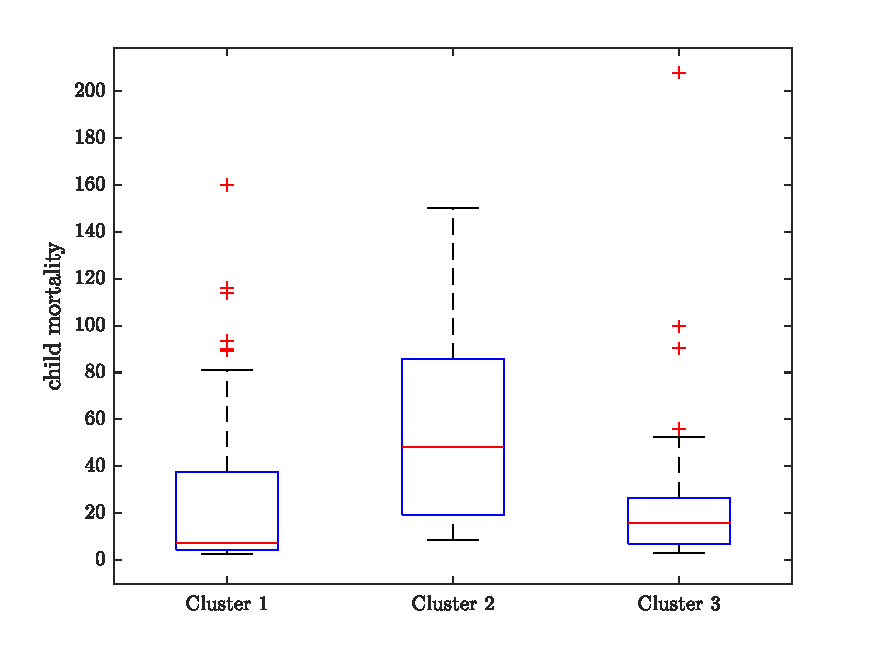
\includegraphics[width=\textwidth]{childmortbox}
    \caption{Child mortality.}
    \label{fig:pbox1}
\end{subfigure}
\hfill
\begin{subfigure}{0.45\textwidth}
    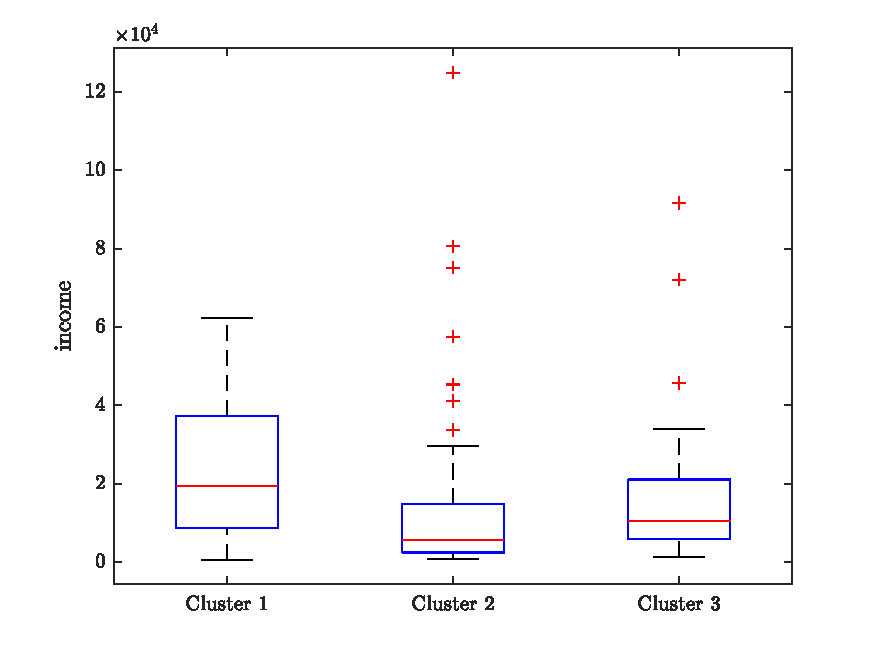
\includegraphics[width=\textwidth]{healthbox}
    \caption{Net income.}
    \label{fig:pbox2}
\end{subfigure}
        
\caption{Death of children under 5 years of age per 1000 live births and net income per person of all the countries within each Cluster.}
\label{fig:pboxes}
\end{figure}
\newpage

By examining the countries within Cluster 1, we can observe that even developed countries such as the United Kingdom are included in this cluster. This suggests that the clustering process and feature engineering\footnote{an alternative is to discard highly correlated data altogether and keep only low-valued correlations; such a case is seen in \cite{notebook}} should be re-evaluated in order to accurately identify which countries are in need of funding.

\begin{verbatim}
           Cluster 1	           Cluster 2	           Cluster 3
          ----------	           ----------	           ----------
         Afghanistan	              Angola	               Benin
        Burkina Faso	             Burundi	             Albania
             Algeria	 Antigua and Barbuda	           Argentina
             Armenia	           Australia	             Austria
             Bahrain	             Belgium	              Brunei
                   .	                   .	                   .
                   .	                   .	                   .
                   .	                   .	                   .
            Tanzania	         Timor-Leste	                Togo
              Uganda	              Zambia	             Uruguay
          Uzbekistan	             Vanuatu	             Vietnam
               Yemen	         Switzerland	United Arab Emirates
      United Kingdom	       United States	           Venezuela
\end{verbatim}

Prima facie evidence suggests that there could be a case for further investigation, to establish whether or not further clustering analysis should be put in hand. Nevertheless, it should be stressed that, an unsupervised analysis is limited and relevant facts could be difficult to establish with any degree of certainty.

\printbibliography

\section*{Appendix A}

According to the World Bank, low income is defined as a gross national income (GNI) per capita of less than \$1,035 per year, while high child mortality is defined as a mortality rate of more than 43 deaths per 1,000 live births. Countries with low income and high child mortality rates tend to have less developed economies and weaker healthcare systems, which can contribute to higher mortality rates among children.

Many factors can contribute to low income and high child mortality in a country, including poverty, lack of access to education and healthcare, lack of infrastructure and resources, and political instability. Developing countries often face these challenges to a greater extent than developed countries, which can lead to higher rates of child mortality and lower levels of economic development.

Several sources discuss the relationship between low income and high child mortality, including:
\begin{itemize}
\item The World Health Organization (WHO) states that "poverty is the single greatest threat to child survival" and that "most of the 10.6 million deaths among children under five occur in developing countries." (\url{https://www.who.int/child_adolescent_health/topics/poverty/en/})
\item The World Bank's World Development Indicators database provides data on income levels and child mortality rates for countries around the world. (\url{https://data.worldbank.org/indicator/SP.DYN.IMRT.IN})
\item The United Nations Children's Fund (UNICEF) reports that "more than half of all child deaths occur in just five countries – India, Nigeria, Pakistan, Democratic Republic of the Congo and China – with India alone accounting for about one third." (\url{https://www.unicef.org/sowc2014/numbers/})
\end{itemize} 

\section*{Appendix B}

\lstinputlisting[caption = {Clustering analysis script}, label = {lst:script}]{../../runMe.m}
\lstinputlisting[caption = {\matlab function for changing the interpreter of all objects within a figure.}, label = {lst:changeInt}]{../../ChangeInterpreter.m}
\lstinputlisting[caption = {\matlab function for configuring a figure's appearance options.}, label = {lst:pltDim}]{../../PlotDimensions.m}

\end{document}